% !TEX root = ../17-MdQM-Vorlesung.tex
%\section*{Einführung}
\label{Sec:introDataScience}
\subsection{Brief Introduction to Data Science}

\frame{\frametitle{What is Data Science?}
\framesubtitle{Data science is our means of taming unstructured information and gathering insight. - Matthew Mayo, KDnuggets}
\begin{itemize}
\item Interdisciplinary field of
\begin{itemize}
		\item Systems,
		\item Methods and
		\item Processs to extract insight or knowledge from data.
\end{itemize}
\item Term coined in 2001, gained popularity in 2010
\item Integrates:
\begin{itemize}
		\item Data Engineering
		\item Scientific Method
		\item Mathematics
		\item Statistics
		\item Advanced Computational Methods
		\item Visualisation
		\item Hacker Mindset
		\item Domain Expertise
		\end{itemize}
\end{itemize}
}


\frame{\frametitle{How does Data Science integrate to Mechanical Engineering?}
\framesubtitle{}
\begin{center}
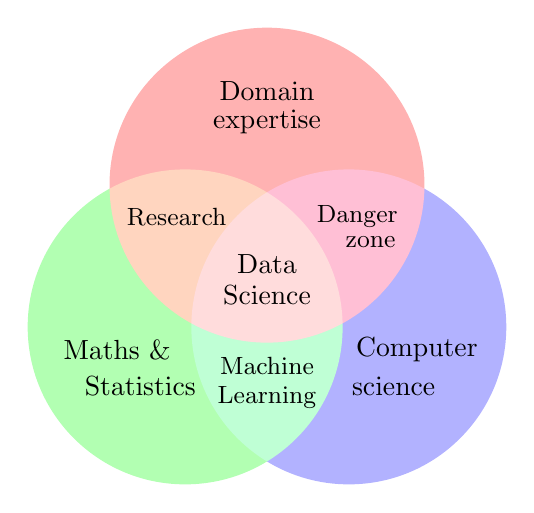
\begin{tikzpicture}
\begin{scope}[blend group=soft light]
\fill[red!30!white] ( 90:1.2) circle (2); 
\fill[green!30!white] (210:1.2) circle (2); 
\fill[blue!30!white] (330:1.2) circle (2); 
\end{scope}
%\node at ( 90:2.6) {Railway}; 
\node at ( 90:2.4) {Domain}; 
\node at ( 90:2.0) {expertise}; 
\node at (205:2.1) {Maths \&};
\node at (220:2.1) {Statistics}; 
\node at (335:2.1) {Computer}; 
\node at (320:2.1) {science}; 
%\node at (0,.4) {Rail};
\node at (0,0.2) {Data};
\node at (0,-.2) {Science};
\node at (270:1.1) {\small Machine};
\node at (270:1.5) {\small Learning};
\node at (145:1.4) {\small Research};
\node at (35:1.4) {\small Danger};
\node at (20:1.4) {\small zone};
\end{tikzpicture}
\end{center}
}

\frame{\frametitle{Why Data Sciene?}
\framesubtitle{Applying the right tools and techniques, you bring more value! }
\begin{columns}[t] 
     \begin{column}[T]{6cm} 
     	\begin{itemize}
     		\item Turn data to information
		\begin{itemize}
		\item Inform decisions
		\item Increase insight
		\end{itemize}
		\item Companies:
		\begin{itemize}
		\item Collect large amounts of data
		\item Do rarely integrate them
		\item Frequently decide based on the ``gut''
		\end{itemize}
     	\end{itemize}
     \end{column}
     	\begin{column}[T]{6cm} 
         	\begin{center}
            		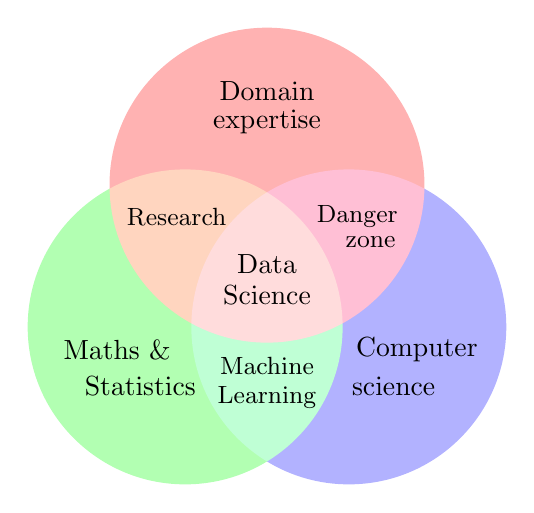
\begin{tikzpicture}
                            \begin{scope}[blend group=soft light]
                            \fill[red!30!white] ( 90:1.2) circle (2); 
                            \fill[green!30!white] (210:1.2) circle (2); 
                            \fill[blue!30!white] (330:1.2) circle (2); 
                            \end{scope}
                            %\node at ( 90:2.6) {Railway}; 
                            \node at ( 90:2.4) {Domain}; 
                            \node at ( 90:2.0) {expertise}; 
                            \node at (205:2.1) {Maths \&};
                            \node at (220:2.1) {Statistics}; 
                            \node at (335:2.1) {Computer}; 
                            \node at (320:2.1) {science}; 
                            %\node at (0,.4) {Rail};
                            \node at (0,0.2) {Data};
                            \node at (0,-.2) {Science};
                            \node at (270:1.1) {\small Machine};
                            \node at (270:1.5) {\small Learning};
                            \node at (145:1.4) {\small Research};
                            \node at (35:1.4) {\small Danger};
                            \node at (20:1.4) {\small zone};
                            \end{tikzpicture}

        		\end{center}
     \end{column}
 \end{columns}
}

\frame{\frametitle{How do you incrase Value with Data Science?}
\framesubtitle{ }
\begin{columns}[t] 
     \begin{column}[T]{6cm} 
     	\begin{itemize}
     		\item Improve decision making
		\begin{itemize}
		\item Empower management
		\item Supply data driven evidence
		\end{itemize}
		\item Identify trends and bring to action
		\item Challenge your colleagues
		\item Find opportunities for improvement
		\item Test decisions
		\item Understand customers
     	\end{itemize}
     \end{column}
     	\begin{column}[T]{6cm} 
         	\begin{center}
            		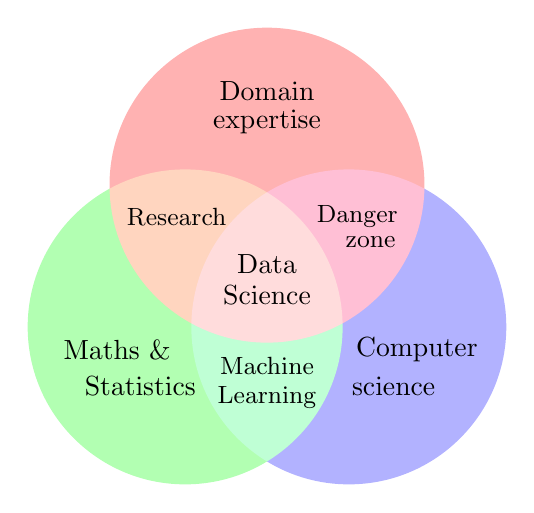
\begin{tikzpicture}
                            \begin{scope}[blend group=soft light]
                            \fill[red!30!white] ( 90:1.2) circle (2); 
                            \fill[green!30!white] (210:1.2) circle (2); 
                            \fill[blue!30!white] (330:1.2) circle (2); 
                            \end{scope}
                            %\node at ( 90:2.6) {Railway}; 
                            \node at ( 90:2.4) {Domain}; 
                            \node at ( 90:2.0) {expertise}; 
                            \node at (205:2.1) {Maths \&};
                            \node at (220:2.1) {Statistics}; 
                            \node at (335:2.1) {Computer}; 
                            \node at (320:2.1) {science}; 
                            %\node at (0,.4) {Rail};
                            \node at (0,0.2) {Data};
                            \node at (0,-.2) {Science};
                            \node at (270:1.1) {\small Machine};
                            \node at (270:1.5) {\small Learning};
                            \node at (145:1.4) {\small Research};
                            \node at (35:1.4) {\small Danger};
                            \node at (20:1.4) {\small zone};
                            \end{tikzpicture}

        		\end{center}
     \end{column}
 \end{columns}
}

\frame{\frametitle{The data science process}
\framesubtitle{}
         	\begin{center}
            		\includegraphics[width=0.8\textwidth]{DataScienceProcess}\source{Source: Farcaster/English Wikipedia}
        		\end{center}
   }

\frame{\frametitle{How to get started}
\framesubtitle{}
\begin{itemize}
\item Set up your system. 
\begin{itemize}
		\item Install Anaconda to obtain Python/Jupyter
		\item Set up a free education account with github.com
		\item Install the app for your operating system
		\end{itemize}
\item Acquire data: start with popular open data sets. Get your company to make data accessible.
\item Ingest and transform: figure out the formats and sizes of your data. Find appropriate ways to import or access them.
\item Explore the data. Do you already find patterns from just plotting them?
\item Try your ``toolbox'' of methods (or a subset of it that sounds promising).
\item Visualise the results. Make your findings convincing to others: colleagues, managers, customers etc.
\end{itemize}
}


